% Section Signal Pre-processing
% !TEX root = ../../main.tex

\section{Signal pro-processing and sensor fusion for timed patterns}
  Describe how data is collected and processed, the form of the data (continuous to discrete, amplitude, energy, frequencies, etc).
  Include feature extraction, like PCA, FFT, energy, mean, but discuss it further in subsection.
  Only the concepts will be explained and the scheme of the computations (or simply formulas), no precise implementations.
  Mention only shortly with meaning, no further explanation.

  --------


    \subsection{Signal fusion}
    Signal fusion is a broad field of research and application and many different interpretations exist.
    The function and interpretation used in this thesis follows the definition from \cite{elmenreich2001introduction}, stating:
    \begin{center}
      \textbf{Sensor fusion} is the combining of sensory data or data derived from sensory data such that the resulting information is in some sense better than would be possible when these sources were used individually.
    \end{center}
    This can essentialy be considered as a form of synergy, in which the combination of the sensors provide more information than the sum of the raw output.
    For the application of this thesis we will focus on direct fusion of raw data, which can be applied to both homogeneous and heterogeneous sensors.
    The fusion stage will combine the data into a single representation, which can be interpreted by the controlling system.
    This differs from mere multisensor integration, in which the controlling system is responsible for processing and interpreting the data from different sources.
    Figure \ref{fig:sensor_fusion} shows the difference.

    \begin{figure}[htbp]
      \centering
        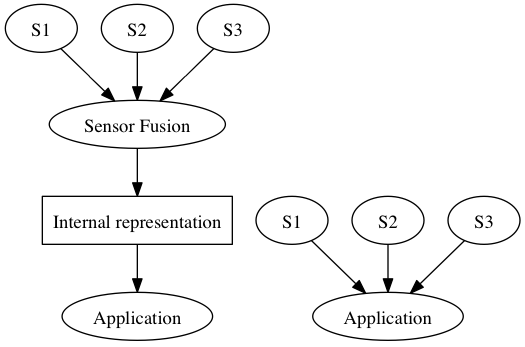
\includegraphics{./Figures/graphs/sensor_fusion.png}
        % \rule{35em}{0.5pt}
      \caption[K-means]{On the left \emph{Sensor Fusion} and on the right \emph{Multisensor integration}}
      \label{fig:sensor_fusion}
    \end{figure}

    Using the single representation, the computational and system complexity can be reduced.
    The representation forms a standardized and normalized interface from the sensors to the system, which create independence and modularity of sensors.
    Other benefits as a result from sensor fusion include \cite{elmenreich2001introduction}:
    \begin{itemize}
      \item \textbf{Robustness en reliability:} When the system incorporates multiple sensors as redundancy, the system becomes more stable in case of partial failure.
      \item \textbf{Extended spatial and temporal coverage:} With multiple sensors a broader spectrum can be analyzed, both in the case of homogeneous and heterogeneous combinations.
      \item \textbf{Increases precision:} Sensors typically have a range and domain of measurements.
      By combining a set of heterogeneous sensors, the overall range of observervation is increased.
      \item \textbf{Reduced ambiguity and uncertainty:} In case of high uncertainty about a observation, the observation of other sensors can confirm it.
    \end{itemize}

    Sensor fusion can be applied on multiple levels. A rough diversion over three levels is:
    \begin{itemize}
      \item \textbf{Low-level:} Raw sensor data is combined which is considered to be more informative than the original sources.
      \item \textbf{Intermediate-level:} Also known as \emph{feature fusion} combines the features which can be extracted from the data.
      See also section \ref{sec:feature_extraction}.
      This data would be applicable to segmentation ***[???].
      \item \textbf{High-level:} Fusion of this level will support decision making, optionally followed by actions taken by the system to the environment or conclusion being drawn from the environment.
    \end{itemize}


    \subsection{Signal smoothing}
    What, why and how.

    \subsection{Feature extraction}
    \label{sec:feature_extraction}
    What, why and how.